\documentclass[stu, a4paper, 12pt, floatsintext]{apa7}

% Title Page Stuff
\title{A Design Report for the Transportation Aircraft Designed in Aircraft Systems Design E3 with a Specific Focus on the Design Aspects Covered by the Author.}
\shorttitle{Individual Design Report}
\leftheader{25/03/25}
\authorsnames{Philip Beswick @00662943}
\authorsaffiliations{The University of Salford}
\course{Aircraft Systems Design E3}
\professor{Dr O K Ariff, Dr Andreea Koreanschi}
\duedate{28/03/25}
\abstract{Some abstract yada yada yada}

% Packages Required
\usepackage{csquotes}
\usepackage[english]{babel}
\usepackage[T1]{fontenc}
\usepackage{mathptmx}
\usepackage{multirow}
\usepackage{graphicx}
\usepackage{booktabs}
\usepackage[style=apa,sortcites=true,sorting=nyt,backend=biber]{biblatex}
\usepackage{pgf-pie}
\usepackage{pgfplots}
\usepackage{paracol}
\usepackage{amsmath}
\usepackage{tocloft}
\usepackage{float}
\usepackage{listings}
\usepackage{gensymb}

\addbibresource{bibliography.bib}

\pgfplotsset{compat=1.18}

% Counts chapters numerically
\setcounter{tocdepth}{5}
\setcounter{secnumdepth}{5}

% Counts equations, figures and tables sequentially depending on the chapter
\numberwithin{figure}{section}
\numberwithin{table}{section}
\numberwithin{equation}{section}

\newcommand{\listequationsname}{\Large List of Equations}
\newlistof{myequations}{equ}{\listequationsname}
\newcommand{\myequations}[1]{%
\addcontentsline{equ}{myequations}{\protect\numberline{\theequation}#1}\par}
\setlength{\cftmyequationsnumwidth}{2.5em}% Width of equation number in List of Equations

% Makes sure LaTeX knows where we are :D
\DeclareLanguageMapping{british}{british-apa}

\begin{document}

\maketitle{} % Generates the title page

\tableofcontents

\newpage

\addcontentsline{toc}{subsection}{List of Figures}
\listoffigures
\addcontentsline{toc}{subsection}{List of Tables}
\listoftables
\addcontentsline{toc}{subsection}{List of Equations}
\listofmyequations

%%% Contents of report go here %%%
\newpage

\section{Introduction}
\section{Overview of Group Design and Market Survey}
\subsection{Market Survey}
\subsection{Design Overview}
\section{Primary Tasks}
\subsection{Initial Weight Estimation}
Once the aircraft concept had been completed and unanimously agreed to by the design team, the first task was to estimate the weights. As a reminder, the aircraft was designed to transport specialist cargo, such as medical supplies, and crew into disaster zones. To do this, the aircraft needs to:
\begin{enumerate}
    \item Have a high payload weight fraction and, 
    \item Operate from short, improvised airfields.
\end{enumerate}

Therefore, the aircraft must weigh as little as possible while generating as much lift as possible with its wings. The goal of this element of the design is to tackle the first of those two characteristics. 

It is well known that there is a complex relationship between aircraft range and weight. Logically, two aircraft of identical design will need different amounts of fuel depending on the distance they intend to travel. Therefore, it was quickly decided that aircraft range would not be a factor of primary concern. The aircraft is designed to transport specialty cargo into areas in need of immediate help, and it would be exceptionally useful if help cannot arrive by other methods of transportation such as road, rail or sea. The aircraft only needs to operate relatively short distances to and from a central hub or distribution centre to deliver aid to a local population. 

The following parameters must be known in order to complete the weight estimation:
\begin{enumerate}
    \item Range (km)
    \item Payload (Pax and Cargo)
    \item Power to Weight (P/W) Ratio of the Engine (kW/kN)
    \item Specific Fuel Capacity (SFC) of the Engine ((N/s)/kW)
    \item Wing Aspect Ratio
    \item Fuselage Diameter/Length
    \item Weight per Pax (kg)
\end{enumerate}

Since the aircraft aims to primarily deliver aid supplies rather than transport people, the parameters were slightly modified to account for pallets of cargo that are one cubic meter in size, each capable of carrying 500kg. In addition to the cargo, the aircraft still aims to transport a small number of passengers; this was decided to be seven people maximum.

The parameters related to the engine (P/W and SFC) were taken from known data for the engine selected to power the aircraft, specifically the Pratt and Whitney 127G. The mass of an average person was approximated to be 90kg, and the fuselage D/L was taken to be 0.13. The two parameters not yet discussed, aspect ratio and range, were the most changeable as the design process continued. In total, 10 different initial weight estimations were conducted, with different parameters, to settle on the most acceptable outcome, which will shortly be presented, but the final value for aspect ratio was taken to be 9, and range to be taken at 1000km (it was decided that this would be sufficient to transport supplies short distances into relief areas). Table 3.1 shows the final design values for weight estimation. 

\begin{table}[]
    \centering
    \caption{Final values for weight estimation}
    \label{tab:weight_estimation_table}
    \begin{tabular}{@{}ccccccccc@{}}
    \toprule
    \textbf{Range} & \multicolumn{2}{c}{\textbf{Payload}} & \textbf{P/W} & \textbf{SFC} & \textbf{Aspect Ratio} & \textbf{D/L} & \multicolumn{2}{c}{\textbf{Payload Masses}} \\ \midrule
    km           & Pax             & Pallets            & kW/kN        & (N/s)kW      &                       &              & Pax (kg)           & Pallets (kg)           \\
    1000           & 7               & 4                  & 17.1         & 0.00076      & 9                     & 0.13         & 90                 & 500                    \\ \bottomrule
    \end{tabular}
\end{table}

Before estimating the aircraft’s weight, the fuselage’s length, breadth and depth can be estimated by the following equations, where $x_p$ is the number of passengers and $x_c$ is the number of pallets (or crates): 
\begin{equation}
    Length = 10+0.237x_p + 1.2x_c \, ,
\end{equation}
\myequations{Equation to find the fuselage length.}
\begin{equation}
    Depth = Length \times {{D}\over{L}} \, ,
\end{equation}
\myequations{Equation to find the fuselage depth.}
\begin{equation}
    Breadth = Length \times {{D}\over{L}} \, ,
\end{equation}
\myequations{Equation to find the fuselage breadth.}

With these equations in mind, the fuselage can therefore be estimated, with the results shown in Table 3.2. 

\begin{table}[]
    \centering
    \caption{This table shows the estimated values for the fuselage.}
    \label{tab:fuselage_estimate}
    \begin{tabular}{@{}ccc@{}}
    \toprule
    \textbf{Length (m)} & \textbf{Breadth (m)} & \textbf{Depth (m)} \\ \midrule
    16.62               & 2.2                  & 2.2                \\ \bottomrule
    \end{tabular}
\end{table}

These values can then be used as a basis when the fuselage design is considered later in the design process. The fuel fraction, however, can now be calculated by the following equation: 
\begin{equation}
    ff = 1.046-e^{-0.3504 \times SFC\times {{Range}\over{\sqrt{AR}}}} \, ,
\end{equation}
\myequations{Equation to find the fuel fraction.}

When this equation is applied to the values found in Table 3.1, the fuel fraction obtained is 0.131, rounded to 3 decimal places. This means that roughly 13\% of the aircraft's weight will be taken up by only the fuel needed to fly, assuming maximum takeoff weight. Similarly, the payload weight can be found by the equation:
\begin{equation}
    W_p (N) = g(x_p \times 90 + x_c \times 500 ) \, ,
\end{equation}
\myequations{Equation to find the payload weight.}

Therefore, the payload weight is found to be 24.92kN. Next, the structural weight can be found, which uses the previously defined parameters for fuselage length, breadth and depth. This means that when the fuselage design has been completed, the weights can be re-estimated to find a more precise maximum takeoff weight. Structural weight is found by the following equation:

\begin{equation}
    W_s (N) = 0.15503 \left( L \times {{B \times D}\over{2}} \right)^{1.3909}
\end{equation}
\myequations{Equation to find the structural weight.}

This means that the structural weight was found to be 23.15kN. Finally, the maximum takeoff weight can now be determined by the following equation: 

\begin{equation}
    W_{to} (kN) = {{5+W_p+W_s}\over{0.8-ff}}
\end{equation}

This means that the aircraft's maximum takeoff weight is 84.59kN, which definately falls within the requirements of EASA-Part 25 to be considered a large aeroplane (greater than 5700kg). Ultimately, this is a good design weight for the aircraft as it falls at the lower end of all the aircraft previously discussed in the market survey, while still being able to carry a sufficiently large payload weight. 

\subsection{Centre of Gravity}
Once the aircraft’s wings, fuselage, and weights have been estimated, balancing the centre of gravity is an excellent way to confirm whether the design choices up to that point were suitable. In addition, EASA Part 25 sets out several key parameters in order for the aircraft to be certifiable, most notably that the centre of gravity’s position must be no more than 50\% of the mean aerodynamic chord or less than 25\% of the mean aerodynamic chord. Furthermore, this must be true in both standard and extreme loading conditions to ensure the flight crew can fly the aircraft with relative ease. 

With this in mind, while noting the aircraft’s initial geometry and layout, the centre of gravity positions can be calculated; this was completed using the moment method, with the reference point taken as the aircraft’s nose.  
\begin{equation}
    X_{CG} = \sum \left( {{m_xx}\over{m_{Total}}} \right) \, ,
\end{equation}
\myequations{Equation to find the aircraft's centre of gravity.}
Where $m_x$ is the mass of a specific component and $x$ is the distance of that component from the datum. $m_{Total}$ is the total mass of all components onboard the aircraft.

Table 3.3 shows the values used to calculate $X_{CG}$ assuming maximum fuel and payload. The values given for $m_x$ are as fractions of the aircraft’s maximum takeoff weight.

\begin{table}[H]
    \centering
    \caption{A table showing the weight fraction of all components onboard the aircraft and their respective position relative to the nose of the aircraft. }
    \label{tab:cg_table}
    \begin{tabular}{@{}lll@{}}
    \toprule
    Component          & $m_x$ (Kg)                      & $x$ (m) \\ \midrule
    Wing               & {\color[HTML]{000000} 0.072472} & 7.29    \\
    Fuselage           & 0.17343                         & 6.65    \\
    Tailplane          & 0.01462                         & 15.08   \\
    Fin                & 0.01389                         & 14.35   \\
    Main Undercarriage & 0.03586                         & 8.04    \\
    Nose Undercarriage & 0.01206                         & 2.97    \\
    Flying Controls    & 0.01715                         & 7.11    \\
    Engine Pod         & 0.01833                         & 5.97    \\
    Engine Installed   & 0.10689                         & 5.55    \\
    Airframe           & 0.14                            & 8.31    \\
    Fuel               & 0.13094                         & 7.17    \\
    Payload            & 0.23256                         & 5.84    \\ \bottomrule
    \end{tabular}
\end{table}

Therefore, when applying Equation 3.8, the centre of gravity position is found to be 6.93m from the aircraft’s nose.

At this stage, it's important to consider how some components' mass will change in flight while others will not. For example, the mass of the aircraft's fuel tanks will decrease during the flight as fuel is burned. However, an aircraft's undercarriage will remain at a constant weight throughout the flight. This is an important consideration to make when tweaking component positions in order to gain a suitable $X_{CG}$ position.

Once the position of the centre of gravity is known, relative to the aircraft’s nose, it is vital to find the position of the centre of gravity in terms of the aircraft’s mean aerodynamic chord (MAC). This can be done using the following relationship:

\begin{equation}
    X_{CG_{MAC}} = {{X_{CG}-X_{MAC_{LE}}}\over{MAC}} \, ,
\end{equation}
\myequations{Equation to find the aircraft's centre of gravity as a fraction of MAC.}
Where $X_{MAC_{LE}}$ is the position of the leading edge of the mean aerodynamic chord and $MAC$ is the length of the mean aerodynamic chord. Therefore, the position of the centre of gravity, as a fraction of the mean aerodynamic chord, is given to be 0.31. This value is within the limits that were previously discussed. Yet, this calculation was only completed for one loading condition, maximum fuel capacity and maximum payload. 

To remain completely compliant with EASA Part-25, this process was repeated for several loading conditions, specifically decreasing fuel by 10\% until there was no fuel left for five different payload configurations. The output for these calculations are plotted on the graph shown in Figure 3.1. 

\begin{figure}[H]
    \caption{The change in CG Position as Fuel Load Decreases}
    \label{fig:cg_pos_graph}
    \centering
    \resizebox{1.0\textwidth}{!}{%
    \begin{tikzpicture}
        \begin{axis}[
            title={},
            xlabel={CG Position as \% of MAC},
            ylabel={\% of Fuel load onboard},
            xmin=0.2, xmax=0.55,
            ymin=0, ymax=100,
            xtick={0.2, 0.25, 0.3, 0.35, 0.4, 0.45, 0.5, 0.55},
            ytick={0, 10, 20, 30, 40, 50, 60, 70, 80, 90, 100},
            legend pos=north west,
            ymajorgrids=true,
            grid style=dashed,
        ]
        
        \addplot[
            only marks,
            mark=diamond,
            color=blue,
            ]
            coordinates {
                (0.389, 100)
                (0.386, 90)
                (0.383, 80)
                (0.378, 70)
                (0.373, 60)
                (0.367, 50)
                (0.36, 40)
                (0.35, 30)
                (0.337, 20)
                (0.32, 10)
                (0.294, 0)                                           
            };
        \addplot[
            only marks,
            color=orange,
            mark=square,
            ]
            coordinates {
                (0.4, 100)
                (0.398, 90)
                (0.395, 80)
                (0.392, 70)
                (0.388, 60)
                (0.383, 50)
                (0.377, 40)
                (0.37, 30)
                (0.36, 20)
                (0.346, 10)
                (0.325, 0)                                             
            };
        \addplot[
            only marks,
            color=green,
            mark=triangle,
            ]
            coordinates {
                (0.411, 100)
                (0.41, 90)
                (0.408, 80)
                (0.406, 70)
                (0.403, 60)
                (0.4, 50)
                (0.396, 40)
                (0.391, 30)
                (0.384, 20)
                (0.375, 10)
                (0.36, 0)                                             
            };
        \addplot[
            only marks,
            color=cyan,
            mark=pentagon,
            ]
            coordinates {
                (0.423, 100)
                (0.422, 90)
                (0.421, 80)
                (0.42, 70)
                (0.419, 60)
                (0.418, 50)
                (0.416, 40)
                (0.414, 30)
                (0.411, 20)
                (0.406, 10)
                (0.399, 0)                                              
            };
        \addplot[
            only marks,
            color=black,
            mark=+,
            ]
            coordinates {
                (0.434, 100)
                (0.435, 90)
                (0.435, 80)
                (0.435, 70)
                (0.436, 60)
                (0.437, 50)
                (0.437, 40)
                (0.438, 30)
                (0.44, 20)
                (0.441, 10)
                (0.445, 0)                                             
            };
            \addplot[
                only marks,
                color=brown,
                mark=star,
                ]
                coordinates {
                    (0.447, 100)
                    (0.448, 90)
                    (0.45, 80)
                    (0.451, 70)
                    (0.454, 60)
                    (0.456, 50)
                    (0.46, 40)
                    (0.465, 30)
                    (0.471, 20)
                    (0.481, 10)
                    (0.496, 0)                                                      
                };
            \addplot[
                color=red,
                mark=circle,
                ]
                coordinates {
                    (0.25, 100)
                    (0.25, 90)
                    (0.25, 80)
                    (0.25, 70)
                    (0.25, 60)
                    (0.25, 50)
                    (0.25, 40)
                    (0.25, 30)
                    (0.25, 20)
                    (0.25, 10)
                    (0.25, 0)                                                   
                };
            \addplot[
                color=red,
                mark=circle,
                ]
                coordinates {
                    (0.5, 100)
                    (0.5, 90)
                    (0.5, 80)
                    (0.5, 70)
                    (0.5, 60)
                    (0.5, 50)
                    (0.5, 40)
                    (0.5, 30)
                    (0.5, 20)
                    (0.5, 10)
                    (0.5, 0)                                                    
                };
            \legend{100\% Payload, 80\% Payload, 60\%Payload, 40\% Payload, 20\% Payload, 0\% Payload}
        \end{axis}
    \end{tikzpicture}
    }
\end{figure}

Figure 3.1 ultimately shows that no matter the aircraft's loading configuration, the CG position remains within the acceptable limits imposed in EASA Part-25. This means that the aircraft has been successfully balanced and that the initial aircraft configuration is acceptable and can be built on in further elements, such as the design of the tailplane and undercarriage. 

Throughout the design process, the CG was constantly tweaked. For example, after completing the fin and tailplane design, more accurate values for tailplane weight and position could be used and implemented in the CG balancing method. This meant that the overall aircraft balancing was constantly being tweaked by slightly moving components with constant weight throughout the flight. The values discussed in this report represent the final values once the design had been completed.  

\subsection{Environmental Control Systems}
Environmental Control systems are crucial to ensure that passengers remain not only comfortable but alive during extended periods at high altitudes. Of course, the aircraft that is being designed is primarily for the transportation of equipment and supplies, but even then, they must be kept at a regulated temperature to ensure that they are free from damage when ready for use. While EASA does not have any particular requirements for environmental control systems, most modern aircraft maintain approximately 10 cubic feet per minute per passenger. This will be a design goal that is kept in mind throughout this process. 

The following two subsections are dedicated to evaluating the fuselage’s skin temperature in various conditions so that heat loading can be calculated for the aircraft in those same conditions. 
\subsubsection{Airfield Condition}
When aircraft are on the ground at an airfield, the cabin temperature will be maintained to create a comfortable environment. For the purposes of these calculations, two extreme conditions will be considered: a hot day ($45 \degree$) without wind and a cold day ($-20 \degree$) without wind. These two conditions will see the environmental control systems work at their hardest, as in the presence of wind, some natural cooling will occur due to decreased fuselage skin temperature. The following parameters are used in this set of calculations:
\begin{table}[]
    \centering
    \caption{This table shows the parameters used when calculating the skin temperature on hot and cold days}
    \label{tab:ecs_airfield_parameters}
    \begin{tabular}{@{}cc@{}}
    \toprule
    Skin Temperature          & $T_s$ \\ 
    Cabin Temperature         & $T_c$ \\
    Ambient Temperature       & $T_1$ \\
    Heat Transfer Coefficient & $U_f$ \\ \bottomrule
    \end{tabular}
\end{table}
These parameters are then applied to Equations 3.10 and 3.11 for a cold and hot day, respectively, where $U_f$ takes the value of 2.44. 
\begin{equation}
    1.25(T_s-T_1)^{1.33} + U_f(T_s-T_c) = 0 \, ,
\end{equation}
\myequations{Airfield Condition - Cold Day Equation to find $T_s$}
\begin{equation}
    1.25(T_s-T_1)^{1.33} + U_f(T_s-T_c) = 90 \, ,
\end{equation}
\myequations{Airfield Condition - Hot Day Equation to find $T_s$}

On both days, the objective is to solve the equations for $T_s$ by iteration so that the left-hand side is approximately equal to their respective values. After much mathematics, it was found that on a hot day, the value of $T_s$ is roughly equal to $50.2905\degree C$ and on a cold day, the value of $T_s$ is approximately $-1.439\degree C$. An example of these iterative calculations can be seen in in Figures 3.2 (hot day) and Figures 3.3 (cold day).

\begin{figure}[H]
    \caption{The iterative process used to find the value of $T_s$ on a hot day, in airfield condition.}
    \label{fig:ecs_hot}
    \centering
    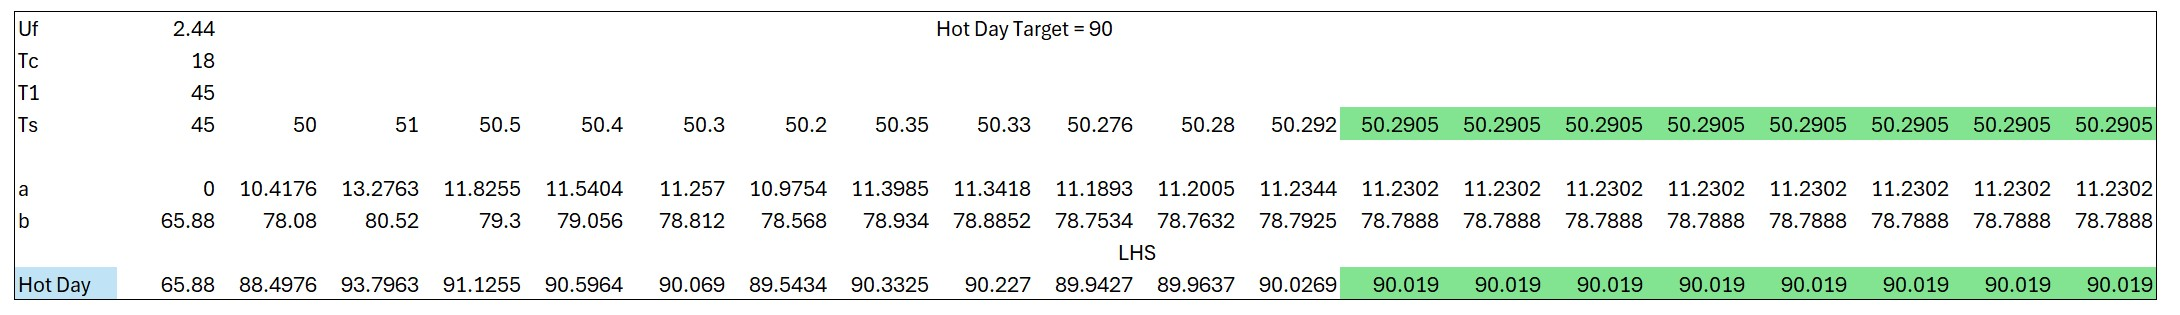
\includegraphics[width=1.1\textwidth]{pictures/ECS_hot_iteration.jpg}
\end{figure}

\begin{figure}[H]
    \caption{The iterative process used to find the value of $T_s$ on a cold day, in airfield condition.}
    \label{fig:ecs_cold}
    \centering
    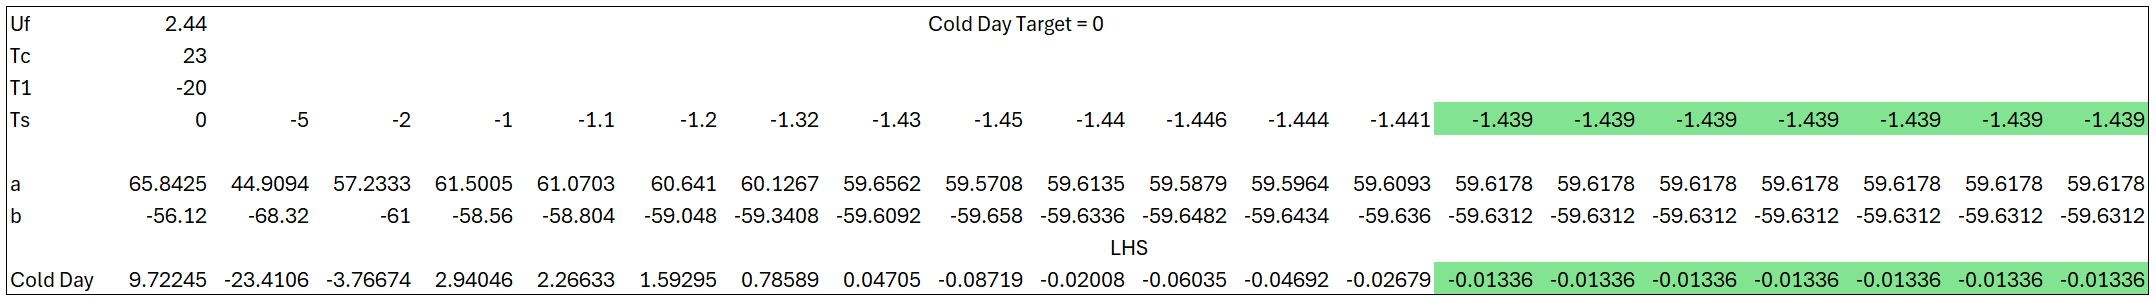
\includegraphics[width=1.1\textwidth]{pictures/ECS_cold_iteration.jpg}
\end{figure}

\subsubsection{Inflight Condition}
When calculating a value for $T_s$ in flight, the mathematical approach is much simpler, as no iterative processes are needed, unlike in the airfield condition. However, it is much more calculation heavy, as the skin temperature will depend on both the aircraft’s cruising speed and altitude. In flight, the heat transfer through the cabin walls is convected to flow around the aircraft. The mathematical expression for this involves Reynold’s analogy between heat transfer and skin friction, which is expressed in terms of the Stanton Number, $S_t$, as seen in Equation 3.12.  
\begin{equation}
    S_t = {{q}\over{\rho u C_p (T_r-T_s)}} \, ,
\end{equation}
\myequations{Equation for Stanton Number $T_s$.}

Where $q$ is equal to the heat transfer per unit area of skin and $T_r$ is the recovery temperature of the skin surface. The equation for $T_r$ is seen in Equation 3.13. In addition, $q$ can be expressed by Equation 3.14, where $S_f$ is the fuselage surface area where heat transfer takes place.

\begin{equation}
    T_r = T_1 (1+0.18M^2) \, ,
\end{equation}
\myequations{The equation for the recovery temperature $T_r$.}
\begin{equation}
    q = {{Q}\over{S_f}} = U_f(T_s-T_c) \, ,
\end{equation}
\myequations{The equation for the heat transfer per unit area of skin $q$.}

This means that an equation for $T_s$ can be constructed, assuming that the Stanton number can be evaluated differently. This is the case, as the Stanton number can be found using the relationship between the average skin friction coefficient ($C_F$) and the Prandtl number ($\sigma$), which is normally taken as 0.72 in air, and is shown in Equation 3.15.

\begin{equation}
    S_t = {{C_F}\over{2\sigma ^{{2}\over{3}}}} \, ,
\end{equation}
\myequations{The equation for the Stanton Number in terms of $C_F$ and $\sigma$.}

The average skin friction coefficient can be found using the Prandtl-Schlichting relationship (Equation 3.17), using the Reynold's number based on fuselage length ($R_L$), which is given by Equation 3.16.

\begin{equation}
    R_L = {{\rho uL}\over{\mu}} \, ,
\end{equation}
\myequations{Equation based for the Reynolds number based on the Fuselage length.}
\begin{equation}
    C_F = 0.455(1-0.1M)(log_{10}R_L)^{-2.58} \, ,
\end{equation}
Finally, this means that the equation for $T_s$ in terms of the Stanton Number can be constructed, as shown in Equation 3.18.

\begin{equation}
    T_S = {{S_t \rho u C_p T_r + U_f T_c}\over{U_f + S_t \rho u C_p}} \, ,
\end{equation}

Therefore, considering a cruising speed of 140 meters per second and a fuselage length of 16.62 meters, $C_F$ can be calculated using Equation 3.17 and a value of 0.002143 is obtained. This means that the Stanton Number can be evaluated using Equation 3.15, and a value of 0.001334 is obtained. At a cruising altitude of twenty thousand feet, the ambient temperature is approximately -27.1$\degree C$, therefore, using Equation 3.13, the recovery temperature is found to be -28.05$\degree C$. Finally, this means that the skin temperature can be obtained using Equation 3.18, assuming the value of $T_c$ is cool at approximately 18$\degree C$, the value of the skin temperature is -27.06$\degree C$.  

\subsubsection{Calculating Heat Load}

Now that the skin temperature values have been obtained in the three different conditions, the heat load of the Environmental Control system can be calculated for each. Heat loading, $Q$, is given by Equation 3.19, where $N_p$ is the number of passengers (7), ${{D}\over{L}}
$ is the drag to lift ratio, ${{W_p}\over{W}}$ is the payload weight to weight ratio, and V is the cruise speed. 

\begin{equation}
    Q = U_f S_f (T_s-T_c) + 450 \times 2.2 + 4.75N_p(39.8-T_c) + 0.001 {{D}\over{L}}{{W_p}\over{W}}VW_p \, ,
\end{equation}

Table 3.5 shows the various heat loads and their respective skin temperatures.

\begin{table}[H]
    \centering
    \caption{This table shows the heat loads for different skin temperatures and conditions}
    \label{tab:ecs_final}
    \begin{tabular}{@{}ccc@{}}
    \toprule
    \textbf{Skin Temperature $T_s$ ($\degree C$} & \textbf{Heat Load Q (W)} & \textbf{Condition} \\ \midrule
    -1.44                                        & -5151.02                 & Airfield Cold      \\
    50.29                                        & 11943.91                 & Airfield Hot       \\
    -27.06                                       & -11170.12                & Cruising           \\ \bottomrule
    \end{tabular}
\end{table}

These values are acceptable for the heat loading of the aircraft’s environmental control system, and if given the chance to do further design work, additional analysis could be performed on what impact these heat loads have on the overall electronic system of the aircraft. 

\section{Secondary Tasks}
\subsection{Aircraft Drag Prediction}
\subsection{Tail and Fin Design}
\section{Design Review}
\section{Group Work Evaluation}
\section{Conclusions}

\section{Appendix}

\addcontentsline{toc}{subsection}{References}
\printbibliography
\end{document}